
\chapter{Method}

\section{Model Intuition}

The model that is developed in this thesis consists of two parts. As a first step, Matrix Factorization (MF) is applied to make a first prediction on the missing drug target pairs. MF predicts the missing values based only on the observations in the training dataset and does not take additional features of the drugs and targets into account. This is where the second part of the model, Continuous Conditional Random Fields (CCRF) comes into play. The CCRF gets the similarity matrices of the drugs and targets as input, together with the training dataset and the predictions that were made by MF on the training dataset. The intuition behind the CCRF is to predict missing values based on three parameters $\alpha$, $\beta_1$, $\beta_2$ which represent respectively:
\begin{itemize}
\item $\alpha$: the \textit{trustworthiness} of the MF prediction. 
\item $\beta_1$: how much can be interpolated between drug-drug pairs with high similarity scores in the drug similarity matrix.
\item $\beta_2$: how much can be interpolated between target-target pairs with high similarity scores in the target similarity matrix.
\end{itemize}

The two parts of the model, MF and CCRF are described first separately and then in combination in the following sections. Matrix Factorization is described in section \ref{sec:MF}. CCRF is described in more detail in section \ref{sec:CCRF}. Both, MF and CCRF are explained by first giving a short overview, then explaining the parameter learning step and finally describing how missing values can be predicted (the inference step).
The combination of the two models (MF and CCRF) is described in section \ref{sec:MFCCRF}. This thesis focuses mainly on the CCRF part of the MF+CCRF model. Before going into the model details, section \ref{sec:Notation} gives an overview of the used notation.

\subsection{Notation}
\label{sec:Notation}
Let $D$ and $T$ denote sets of drugs and targets respectively. Let $R \in \mathbb{R} ^{|D| \times |T|}$ denote a drug-target interaction matrix, where the rows represent the drugs in $D$ and the columns represent the targets in $T$. $R$ contains missing values for drug-target pairs for which the interaction strength is unknown and real values representing the interaction strength for drug-target pairs whose binding affinity was measured in wetlab experiments. The known values in $R$ serve as training data for the developed model. Furter, let $S_D \in \mathbb{R}^{|D| \times |D|}$ and $S_T \in \mathbb{R}^{|T| \times |T|}$ denote matrices containing similarity scores for the drugs $D$ and targets $T$ respectively. The interaction data and similarity scores can be of different kind as described in section [insert reference to data section].  In the \textit{drug target interaction prediction} task, the number of missing values in $R$ usually outweights the number of known interactions and $R$ is only sparsely populated (see data section).

\subsection{Matrix Factorization}
\label{sec:MF}
The Matrix Factorization (MF) technique has been demonstrated to be effective specially for personalized recommendation tasks \cite{Koren:2009:MFT:1608565.1608614} and it has been previously applied for drug target interaction prediction \cite{liu2016neighborhood}, \cite{ezzat2016drug}, \cite{gonen2013kernelized}. Here, the MF technique is utilized in its simplest form, without incorporating the similarity matrices directly as it is done in \cite{liu2016neighborhood} and \cite{gonen2013kernelized}. MF is a process in which the sparsely filled training matrix $R$ is approximated by the product of two factor matrices $P \in \mathbb{R}^{k\times |D|}$ and $Q \in \mathbb{R}^{k\times |T|}$ as described in the following two sections.

\subsubsection{Parameter Learning}

The factor matrices $P$ and $Q$ are learned by minimizing the regularized squared error on the set of known affinities $\kappa$:
\begin{equation}
\min\limits_{Q,P}{\sum\limits_{(d_i,t_j)\in \kappa} (a_{i,j}-q_i^Tp_j)^2} + \lambda (||p||^2 + ||q||^2)
\end{equation}
The term $(a_{i,j}-q_i^Tp_j)^2$ represents the fitting of the learned parameters to the previously observed binding affinites. The term $\lambda (||p||^2 + ||q||^2)$ penalizes the magnitudes of the learned parameters to prevent overfitting and the constant $\lambda$ controls the extend of overfitting.
The above optimization problem can be solved by stochastic gradient descent as described in \cite{Koren:2009:MFT:1608565.1608614}:
The algorithm loops through all pairs $(d_i, t_j)$ in $R$ for which the binding affinity is known, computes the current prediction for $(d_i, t_j)$ and computes the associated prediction error as:
\begin{equation}
e_{i,j} = r_{i,j} - p_i^Tq_j
\end{equation}
where $p_i$ denotes the $i$th column of $P$ and $q_j$ denotes the $j$th column of $Q$. The columns of $P$ and $Q$ are then modified in the opposite direction of the gradient:
\begin{equation}
p_i:= q_i + \gamma (e_{i,j} p_j - \lambda q_i)
\end{equation}
\begin{equation}
q_j:=p_i + \gamma (e_{i,j} p_i - \lambda q_j)
\end{equation}
where $\gamma$ is a constant specifying the magnitude of the update.

\subsubsection{Inference}

With learned matrices $P$ and $Q$, a missing affinity of drug-target pair $(d_i, t_j)$ in $R$ can be predicted by the inner product of the $i$th column of $P$ and the $j$th column of $Q$. A matrix $R'$ with predictions for all drug-target pairs can be computed as:
\begin{equation}
R' = P^TQ
\end{equation}

\subsection{Continuous Conditional Random Fields}
\label{sec:CCRF}

Conditional Random Fields were originally developed for the task of segmenting and labeling sequence data \cite{lafferty2001conditional}. In contrast to predicting continuous values as for drug target binding affinities, the original formulation predicts a label vector $Y$, where all components of $Y_i$ are assumed to range over a finite label alphabet $\mathcal{Y}$. For the task of classifying whether or not a drug-target pair is interacting, CRFs were applied previously \cite{yang2014drug}.

%(non-continuous) Conditional Random Fields were applied successfully for tasks, such as ...

To the best of my knowledge, the continuous variant of Conditional Random fields were first introduced by \cite{qin2009global} for ranking tasks in document retrieval systems. An other application of CCRFS for recommender systems can be found in \cite{xin2009social}. The problem formulation in \cite{xin2009social} is very similar to the problem of drug-target interaction prediction. However the formulation in \cite{xin2009social} requires taking a Gibbs-sample of the distribution defined through the CCRF in each update step during parameter learning. Although with the drawback of reducing the feasible size of the graphical model, \cite{baltruvsaitis2013dimensional} presents a closed form solution for the parameter learning and inference step. This closed formulation of the CCRF is applied for the model that is used in this thesis. The following sections formally describe the CCRF and explain the perameter learning and the inference step.


%In the non-continuous formulation, label sequences $Y$ are modeled as a conditional distribution $P(Y|X)$.

%describe difference to HMMs [In contrast to the generative Hidden Markov Models, defining a joint probability over observation and label sequences, which require to enumerate all possible observation sequences, a conditional model specifies the probabilities of possible label sequences \textbf{given} an observation sequence. Therefore a conditional model does not expend modeling effort on the observations.]

%Conditional Random Fields model a sequence of labels $Y$, given an observation vector $X$ as a conditional probability $P(Y|X)$. In non-continuous CRFs, the components $Y_i$ of $Y$ are assumed to range over a finite label alphabet $\mathcal{Y}$.


\subsubsection{Formal Definition}
Here I will use the same notation as it is presented in \cite{baltruvsaitis2013dimensional}. A CCRF is an undirected graphical model which models a set of output variables $Y=\{y_1,\dots,y_n\}$, $y_i \in \mathbb{R}$ that we wish to predict as $P(Y|X)$ where  $X=\{x_1,\dots,x_n\}$, $x_i \in \mathbb{R}^m$ is a set of observed input variables. The CCRF defines a conditional probability distribution with the density function:
\begin{equation}\label{eq:CCRF_main}
P(Y|X)=\frac{exp(\Psi)}{\int_{-\infty}^{\infty} exp(\Psi) dy}
\end{equation}
\begin{center}
$\Psi=\sum_i \sum\limits_{k=1}^{K_1} \alpha_k f_k(y_i, X) + \sum_{i,j} \sum \limits_{k=1}^{K_2} \beta_k g_k (y_i, y_j,X)$
\end{center}
The term $\int_{-\infty}^{\infty} exp(\Psi) dy$ is a normalization term which makes the probability distribution valid. The $f_k$ terms will be called vertex features and the $g_k$ terms edge features. The feature functions are defined as:
\begin{center}
$f_k(y_i,X) = -(y_i - X_{i,k})^2$\\
$g_k(y_i,y_j,X) = -\frac{1}{2}S_{i,j}^k(y_i - y_j)^2$
\end{center}
Intuitively, the weights $\alpha_k$ on the feature functions $f_k$ represent the reliability of observation $X_{i,k}$ in regard to the true label $y_i$. Here, the observations $X_{i,k}$ can for example represent the predictions of $K_1$ regressors. In the CCRF that is used for the experiments in this thesis $K_1$ is always $K_1=1$ and $X_{i,1}$ represents the initial prediction coming from the Matrix Factorization part of the model.  Edge features $g_k$ represent the dependency between labels $y_i$ and $y_j$ with similarity $S_{i,j}^k, k \in 1,\dots, K_2$. With given drug-drug similarity matrix $S_D$ and target-target similarity matrix $S_T$, $S_{i,j}^1$ and $S_{i,j}^2$ can for example be defined as:
\begin{equation}
\label{simi_1}
S_{i,j}^1 =
\begin{cases}
1, & S_D(i,j) > thresh_d \\
0, & S_D(i,j) < thresh_d
\end{cases} 
\end{equation}
\begin{equation}
\label{simi_2}
S_{i,j}^2 =
\begin{cases}
1, & S_T(i,j) > thresh_t \\
0, & S_T(i,j) < thresh_t
\end{cases} 
\end{equation}
where $thresh_d$ and $thresh_t$ are user defined thresholds. Intuitively, the parameters $\beta_1$ and $\beta_2$ now represent the importance of assigning similar prediction values to drug pairs with similarity larger than $thresh_d$ and of assigning similar prediction values to target pairs with similarity larger than $thresh_t$.

As explained in the following sections, the conditional probability distribution that is defined through the CCRF can be transfomerd into a multivariate Gaussian distribution in closed form, which is a useful property for both learning the weights on the feature functions as well as making predictions for missing values.
\subsubsection{Parameter Learning}

This section describes the parameter learning procedure of the CCRF for quadratic vertex and edge functions as described above. Assume we are given training values $Y=\{y_1,\dots,y_n\}$. Additionally, for each $y_i$ we have given the prediction $X_{i,k}$ that regressor $k$ would have predicted. As explained above, for the model in this thesis we have $K_1=1$ and thus we have only one prediction $X_{i,1}$ for each training data point, which is the Matrix Factorization prediction. Further we have $K_2$ similarity matrices given which in the scope of this thesis are the matrices $S_{i,j}^1$ and $S_{i,j}^2$ as defined in equation \ref{simi_1} and equation \ref{simi_2} respectively. In the learning step, we want to find the $\alpha$ and $\beta$ weights, that optimise the conditional log-likelihood of the CCRF on the training data:

\begin{equation}  
\label{eq:log_likelihood}
L(\alpha,\beta)=\text{log}P(Y|X)
\end{equation}
\begin{equation}  
(\alpha_{opt}, \beta_{opt}) = \argmax_{\alpha, \beta}(L(\alpha,\beta))
\end{equation}
Because this problem is convex \cite{qin2009global}, standard techniques such as stochastic gradient descent can be utilized to determine the optimal parameters $\alpha$ and $\beta$. As described in \cite{baltruvsaitis2013dimensional}, the partial derivatives of \ref{eq:log_likelihood} can be derived by first converting \ref{eq:CCRF_main} into the format of a multivariate Gaussian:

First, the feature functions are pluged into the energy function $\Psi$:

\begin{equation}
\label{learning:Psi}
\begin{split}
& \Psi = \sum\limits_{k=1}^{K1} \alpha_k f_k(y_i, X) + \sum_{i,j} \sum \limits_{k=1}^{K2} \beta_k g_k (y_i, y_j,X) \\
& = -\sum\limits_{k=1}^{K1} \alpha_k (y_i - X_{i,k})^2 - \frac{1}{2} \sum_{i,j} \sum \limits_{k=1}^{K2} \beta_k S_{i,j}^k(y_i-y_j)^2
\end{split}
\end{equation}

For the next step, we first define a diagonal matrix $A$ and a symmetric matrix $B$:
\begin{equation}
A_{i,j}=
\begin{cases}
\sum_{k=1}^{K_1} \alpha_k, & i=j\\
0, & i \neq j
\end{cases}
\end{equation}
\begin{equation}
B_{i,j} = 
\begin{cases}
(\sum_{k=1}^{K_2}\beta_k \sum_{r=1}^{n} S_{i,r}^k) - (\sum_{k=1}^{K_2} \beta_k S_{i,j}^{k}), & i=j \\
-\sum_{k=1}^{K_2} \beta_k S_{i,j}^k, & i \neq j
\end{cases}
\end{equation}
as well as 
\begin{equation}
\Sigma^{-1} = 2(A+B)
\end{equation}
and a vector $\boldsymbol{b}$:
\begin{equation}
\boldsymbol{b}_i = 2 \sum \limits_{k=1}^{K_1} \alpha_k X_{i,k}
\end{equation}
\begin{equation}
\boldsymbol{b} = 2X\alpha
\end{equation}
The factor $\Psi$ in equation \ref{learning:Psi} can then be expressed in terms of $A, B$ and $\boldsymbol{b}$:
First, terms of $\Psi$ containing $\alpha$ parameters are collected:

\begin{equation}
\begin{split}
& -\sum_i \sum \limits_{k=1}^{K_1} \alpha_k(y_i-X_{i,k})^2 \\
& = -\sum_i \sum \limits_{k=1}^{K_1} \alpha_k(y_i^2-2y_iX_{i,k}+X_{i,k}^2) \\
& = -\sum_i \sum \limits_{k=1}^{K_1} \alpha_k y_i^2 + \sum_i \sum\limits_{k=1}^{K_1} \alpha_k 2y_i X_{i,k} - \sum_i \sum\limits_{k=1}^{K_1} \alpha_k X_{i,k}^2\\
& = -y^TAy + y^tb - \sum_i \sum\limits_{k=1}^{K_1} \alpha_k X_{i,k}^2
\end{split}
\end{equation}
Then, terms of $\Psi$ containing $\beta$ parameters are collected:
\begin{equation}
\begin{split}
& -\frac{1}{2}\sum_{i,j}\sum\limits_{k=1}^{K_2}\beta_k S_{i,j}^k(y_i-y_j)^2\\
& = -\frac{1}{2}\sum_{i,j}\sum\limits_{K=1}^{K_2}\beta_k S_{i,j}^k(y_i^2-2y_iy_j+y_j^2)\\
& = -\frac{1}{2}\sum_{i,j}\sum\limits_{K=1}^{K_2}\beta_k S_{i,j}(y_i^2+y_j^2) + \sum_{i,j} \sum\limits_{k=1}^{K_2}\beta_k S_{i,j}^ky_iy_j\\
& =  -\sum\limits_{k=1}^{K_2}\beta_k\sum_{i,j}S_{i,j}^ky_i^2 + \sum\limits_{k=1}^{K_2}\beta_kS_{i,j}^k\sum_{i,j}y_iy_j\\
& = -y^TBy
\end{split}
\end{equation}
Combining these leads to the Gaussian expression of $\Psi$:
\begin{equation}
\Psi=-y^TAy + y^Tb - y^TBy - d = - \frac{1}{2}(y^T\Sigma^{-1}y)+y\Sigma^{-1}\mu - d
\end{equation}
where $d=\sum_i\sum\limits_{k=1}^{K_1}\alpha_kX_{i,k}^2$ and $\mu = \Sigma b$.

\subsubsection{Inference}

As described above, the CCRF can be viewed as a multivariate Gaussian. Therefore, the prediction $Y'$ that maximizes $P(Y'|X)$ is the mean value of the distribution:
\begin{equation}
Y' = \argmax_{Y} P(Y|X) = \mu = \Sigma\boldsymbol{b}
\end{equation}
This way, the CCRF predicts the missing values \textit{as well as} the values already in the training set. In order not to predict the known values anew, the resulting multivariate Gaussian can be conditioned on the training data.

\subsection{MF+CCRF}
\label{sec:MFCCRF}

This section gives an overview of the combined MF+CCRF model. Assume we have a matrix $R \in \mathbb{R} ^{|D| \times |T|}$ given and corresponding similarity matrices $S_D \in \mathbb{R}^{|D| \times |D|}$ and $S_T \in \mathbb{R}^{|T| \times |T|}$ for the drugs $D$ and targets $T$ as described in sec \ref{sec:Notation}. It is our goal to predict the binding affinities of those drug-target pairs in $R$ for which no binding value is given. The given binding affinities serve as training data.

The main part of the MF+CCRF model is on the CCRF part. The purpose of MF is to give a first prediction on the missing drug target pairs which is then refined by the CCRF. The CCRF interpolates between similar drugs and targets, where similarity is defined through the similarity matrices. This interpolation can happen either between two drug-target pairs, where a prediction is made for both pairs or from a known affinity value of one drug-target pair to a pair that is predicted. The CCRF learns the importance of the MF prediction and the importance of the interpolation between drug-target pairs from the training data.
Assume that $Y_{train} = \{y_1, \dots, y_n\}$ is the set of known binding values in $R$. This means that $x_1$ is the MF prediction on training value $y_1$, $x_2$ is the MF prediction on training value $y_2$ and so on. Although the vector $X_{train}$ contains the prediction of MF on the training data itself it should represent the performance of MF on the actual missing values. In order not to overfit the Matrix Factorization model on the training data, when obtaining $X_{train}$ (as this would result in an over optimistic vector $X_{train}$), the training data is partitioned into 5 folds of which 4 folds are used as training data to predict the fold that was left out. The procedure is repeated for each fold to get the complete vector $X_{train}$ as illustrated in figure \ref{fig:ccrf_X}. Each element in $Y_{train}$ and each element in $X_{train}$ correspond to a node of the graphical structure of the CCRF as illustrated in ??. The edges of the graphical model are defined through the similarity matrices of the drugs and targets. One possible way of connecting the nodes is by connecting each drug to its $k$ most similar drugs and similarly connect each target to its $k$ most similar targets. Another way of chosing the edges is by connecting all drugs and targets respectively whose similarity is above a user defined threshold. Following the notation in \ref{sec:CCRF}, we have one initial prediction $X_{train}$ (thus $K_1=1$ as mentioned in \ref{sec:CCRF}). Looking back at equation \ref{eq:CCRF_main}, we see that $K_2$ different similarity matrices $S_{i,j}^k, k \in \{1,\dots,K_2\}$ can be given for the nodes. We can for example choose to learn one parameter $\beta$ for all edges but we can also split the edges into edges that are defined through the drug-drug similarity and edges that are defined through the target-target similarity. In the second case we would learn two edge parameters $\beta_1$ and $\beta_2$. Other variations are of course possible, such as learning separate edge parameters for each drug and target. Figure ?? shows an example, where all drugs and targets are connected to its $k$ nearest neighbors and illustrates the two cases of learning one parameter for all edges and learning two parameters for the drugs and targets respectively. Note that the $S_{i,j}^k$ matrices are of dimension $n \times n$ where $n$ is the number of nodes in the CCRF. For the training step, the number of nodes in the CCRF is $n = Y_{train}$
 and thus $S_{i,j} \in \mathbb{R}^{|Y_{train}| \times |Y_{train}|}$. For the prediction step, the number of nodes in the CCRF is equal to the number of cells in the matrix $R$ and thus $S_{i,j} \in \mathbb{R}^{|D||T| \times |D||T|}$

\begin{figure}
\begin{center}
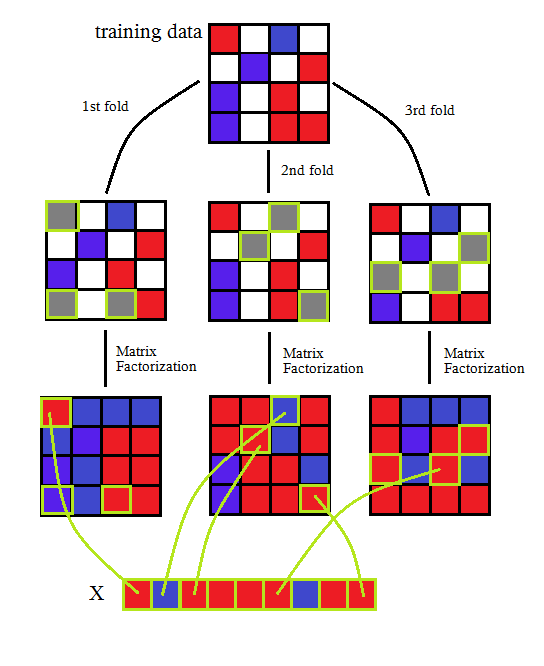
\includegraphics[scale=0.6]{ccrf_X.png}
\end{center}
\caption{Illustration of steps to get vector $X$: The training data is partitioned into k folds. For each fold, the training data is masked and MF predicts all remaining values in the matrix including the masked fold. Vector $X$ is obtained, by combining the predictions of each fold. Note that the vector $X$ represents the predictions of the given matrix values as a vector in row-first order and that the length of the vector $X$ is equal to the number of training observations . In this example, a matrix of 4 drugs and 4 targets with 9 training points is given, thus the length of $X$ is 9.}
\label{fig:ccrf_X}
\end{figure}


\begin{figure}
\begin{center}
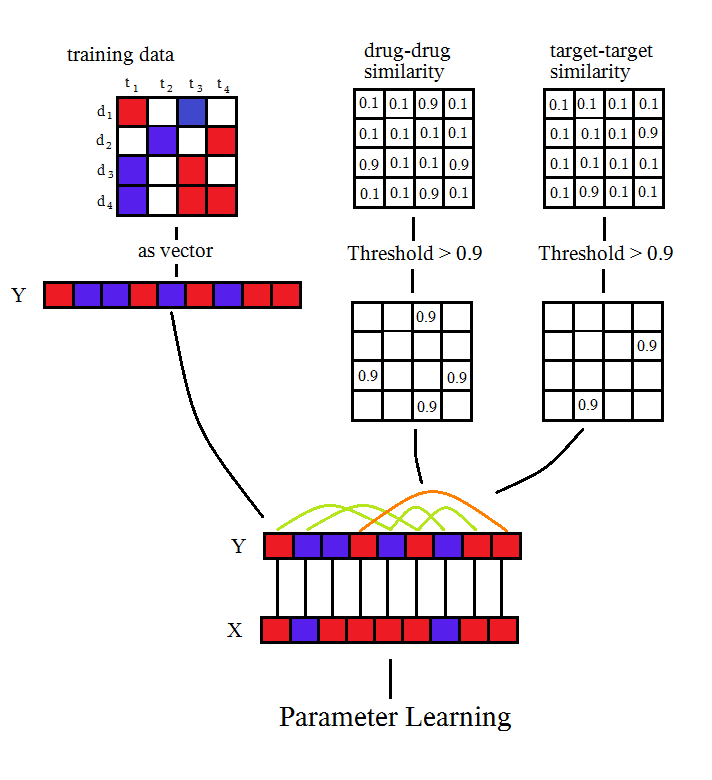
\includegraphics[scale=0.6]{ccrf_input.png}
\end{center}
\caption{Illustration of Parameter Learning: Input for the learning step of the CCRF are the given observations in the drug-target matrix, the vector $X$ that was predicted by MF, and the similarity matrices of the drugs and targets. Here, the given observations are transformed into a vector $Y$ in row-first order (corresponding to vector $X$). The graphical structure of the CCRF is defined by the similarity matrices of the drugs and targets. A threshold $t$ can be applied to connect only those nodes that have a similarity $>t$. In the above example, drugs $(d_1, d_3)$ and $(d_3, d_4$) and targets $(t_2, t_4)$ have similarity scores above the threshold. Thus the nodes $(1,5)$ and $(2,6)$ are connected (because they belong to drugs $(d_1, d_3)$. Further the nodes $(5,7)$ and $(6,8)$ are connected (because they belong to drugs ($d_3, d_4$)) and the nodes $(4,8)$ are connected because they belong to targets $(t_2, t_4)$. One parameter $\alpha$ is learned for the dependece between $Y$ and $X$. Another parameter $\beta_1$ is learned for the dependence between similar drugs (green edges) and a third parameter $\beta_2$ is learned for the dependence between similar targets (orange edges).}
\label{fig:ccrf_X}
\end{figure}


\section{Proof of Concept}

This section serves as a proof of concept for the model that is developed in this thesis. In a first step, a matrix of $n$ rows and $m$ columns is generated which is then partitioned into training and test data ($n$ simulated drugs and $m$ simulated targets). The matrix values are generated, such that the following assumptions are fulfilled:

\begin{itemize}
\item the dataset has underlying latent factors
\item there are certain pairs of columns in the generated dataset, s.th. the pairs of columns have similar values (simulating similar targets).
\end{itemize}

In a second step, a fraction of observations in this generated dataset is masked as test data. The remaining values are used as training data for the MF+CCRF model. The models parameters are trained based on the training data and in the next step the values that were previously masked as test data are predicted. Finally, the performance of this model is evaluated in terms of RMSE and compared to the performance of using only MF or only CCRF.
In the following, each of these steps is documented, starting with the simulation of the data.

\subsection{Data Simulation}
%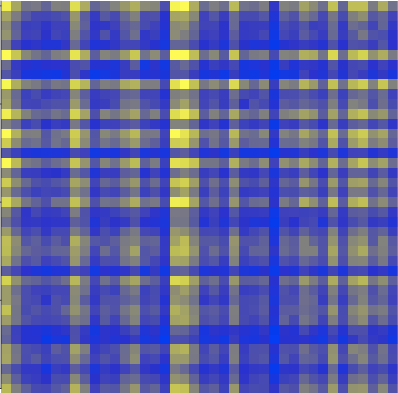
\includegraphics[scale=0.3]{num_lf_mat.png}

A dataset of dimension $m \times n$ ($m$ drugs and $n$ targets) that has underlying latent factors and column-pairs with similar values can be simulating by taking a sample from the distribution that is defined by the CCRF. At first, a matrix $X$ of size $m \times n$ is generated which has only underlying latent factors as shown in figure \ref{fig:numX}. Next, the graphical structure of the CCRF is defined by arbitrarily choosing pairs of columns for which the CCRF distribution should produce similar values. In the CCRF formulation each matrix cell is a node and each node can be adjacent to any other node in the graphical model. Therefore the graphical structure of the CCRF is defined by an adjacency matrix $B$ of size $mn \times mn$. Figure \ref{fig:numStructure} shows an example of a choice of structure for the CCRF.  The values in matrix $X$ are used as node input for the CRF. Next $\alpha$ (importance of the node values) and $\beta$ (importance of the adjacency matrix) are chosen arbitrarily and a sample from the multivariate gaussian distribution that can be derived from the CCRF formulation is taken. This sample is used as the dataset for the numerical experiments. It has both underlying latent factors and the assumption that \textit{similar targets} (which were chosen arbitrarily by defining the matrix $B$) have similar values is fulfilled. Figure \ref{fig:numSample} shows an example of a sample, taken from the multivariate gaussian that is defined by the CCRF where the structure of the model was chosen as described in Figure \ref{fig:numStructure}.

%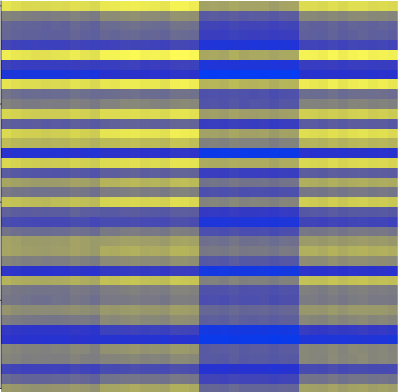
\includegraphics[scale=0.2]{num_lf_crf_mat.png}
%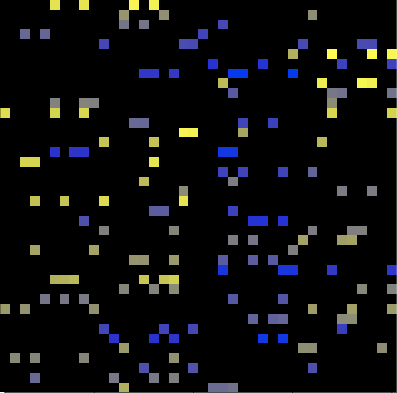
\includegraphics[scale=0.2]{num_train.png}
%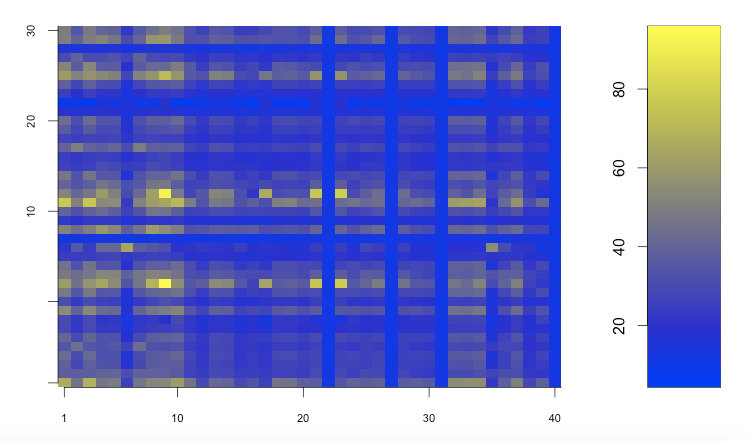
\includegraphics[scale=0.2]{num_pred_mf.png}
%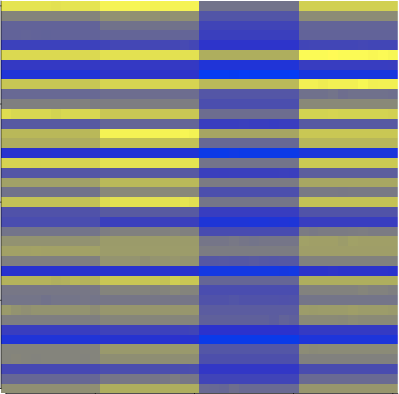
\includegraphics[scale=0.2]{num_pred_mf_crf.png}
\begin{figure}
\begin{center}
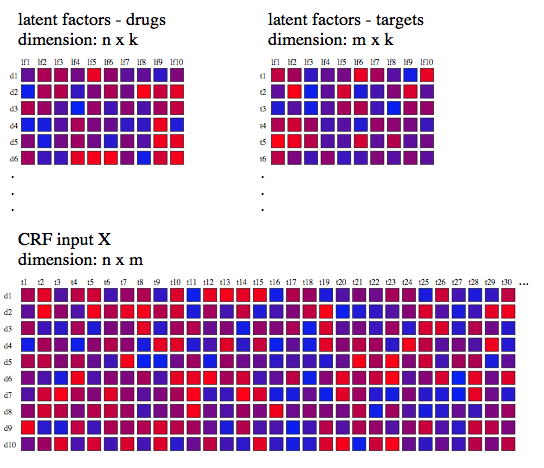
\includegraphics[scale=0.6]{numeric_X.png}
\end{center}
\caption{Sampling matrix $X$ which is used for the node input of the CCRF distribution. First two latent-factor-matrices $LF_d$ and $LF_t$ of dimension $n \times k$ and $m \times k$, where $n$ is the number of drugs, $m$ is the number of targets and $k$ is the number of latent factors (here $k=10$ is chosen arbitrarily) are sampled randomly. $X$ is defined as the product $X=LF_d LF_t^T$ and is used as the values for the node input of the CCRF.}
\label{fig:numX}
\end{figure}

\begin{figure}
\begin{center}
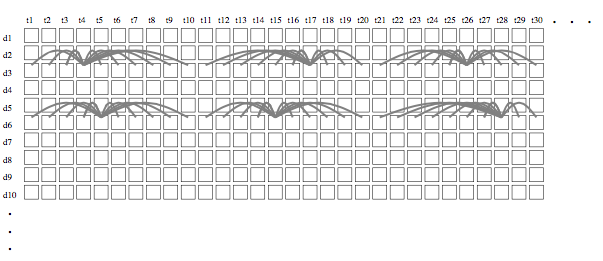
\includegraphics[scale=0.6]{numeric_structure.png}
\end{center}
\caption{Defining the structure of the CRF. Assume each matrix cell is a node of the CCRF. For the numerical experiments, the matrix columns where divided into groups of 10 columns. Each cell in each group was connected to all other cells in the same group, which is illustrated by the archs.}
\label{fig:numStructure}
\end{figure}


\begin{figure}
\begin{center}
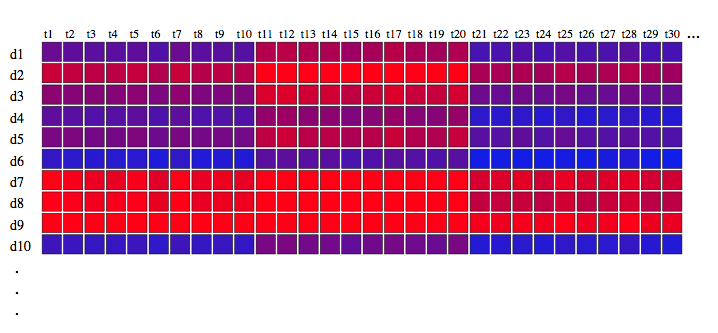
\includegraphics[scale=0.5]{numeric_sample.png}
\end{center}
\caption{Example of a dataset that is sampled from the CCRF when the structure is chosen, such as described in Figure \ref{fig:numStructure}. This dataset has the property that the nodes which are interconnected by the structure of the graphical model have similar values.}
\label{fig:numSample}
\end{figure}

\subsection{Experiments on Simulated Data}

For the numerical experiments a dataset of $n=40$ rows and $m=40$ columns was generated. As described above for the dataset generation, a first dataset $X$ was generated which has only underlying latent factors. Next the CCRF parameters were chosen arbitrarily as $\alpha=1$ and $\beta=2$. The graphical structure of the CCRF was chosen as illustrated in Figure \ref{fig:numStructure}. Next, the corresponding multivariate Gaussian was obtained, by first calculating the covariance matrix $\Sigma$ and mean vector $\mu$ as described in section \ref{sec:CCRF}. A sample from this distribution was taken as the simulated dataset. Next, 150 training values were sampled from the complete dataset. 


